%!TEX program = xelatex
\documentclass[table,aspectratio=169]{beamer}

%\usefonttheme{professionalfonts}
\usepackage[T1]{fontenc}
\renewcommand*\familydefault{\sfdefault}

\usepackage{beamerthemesplit}
\usepackage{graphicx}
\graphicspath{{./Figures/}}

\usepackage{bm,bbm,bbding}
\usepackage{natbib}
\usepackage{siunitx}
\usepackage{texnames}
\usepackage{algorithm,algpseudocode}
\usepackage{multirow}
\usepackage{booktabs}
\usepackage{amsmath}

\definecolor{anti-flashwhite}{rgb}{0.95, 0.95, 0.96}
\definecolor{byzantine}{rgb}{0.74, 0.2, 0.64}
\definecolor{VUWlightgreen}{rgb}{0, .294, .204}
\definecolor{VUWgreen}{rgb}{0, .196, .136}

\usetheme[numbering=fraction]{metropolis}

\setbeamercovered{dynamic}
\setbeamercolor{background canvas}{bg=VUWgreen}
\setbeamercolor{normal text}{fg=anti-flashwhite, bg=VUWgreen}
\setbeamercolor{frametitle}{bg=VUWlightgreen,fg=anti-flashwhite}
\setbeamercolor{footline}{bg=VUWlightgreen}

\makeatletter
\setlength{\metropolis@frametitle@padding}{.5em}% <- default 2.2 ex

\setbeamertemplate{footline}{%
\begin{beamercolorbox}[wd=\textwidth, sep=.2ex]{footline}% <- default 3ex
\usebeamerfont{page number in head/foot}%
\usebeamertemplate*{frame footer}
\hfill%
\usebeamertemplate*{frame numbering}
\end{beamercolorbox}%
}
\makeatother

\setbeamertemplate{frame footer}{\includegraphics[width=1.5cm]{"Logo Offshore Reversed Landscape RGB"}}
\setbeamertemplate{navigation symbols}{}

\AtBeginSubsection[]
{
\begin{frame}
\frametitle{Table of Contents}
\tableofcontents[currentsection,currentsubsection]
\end{frame}
}

\title{Identifying Heterogeneity in SAR Data with New Test Statistics}
\subtitle{No problem is too old, and you don't always need deep learning}
\author{Alejandro C.\ Frery}
\institute{Victoria University of Wellington\\
School of Mathematics and Statistics\\
New Zealand}
\date{November, 2024}

\begin{document}

\setsansfont[BoldFont={Avenir Heavy}]{Avenir Book}

\frame{\titlepage}

\begin{frame}
This is a joint work with Prof.\ Abraão Nascimento and MSc.\ Janeth Alpala (it is part of her PhD project), from Universidade Federal de Pernambuco, Brazil.
\end{frame}

\begin{frame}{Starting point}
\begin{itemize}[<+->]
	\item Synthetic Aperture Radar (SAR) technology is essential for environmental monitoring and disaster management. 
	\item It provides
	images under various conditions, including day or night and adverse weather
	situations~\citep{Moreira2013,Mu2019}. 
	\item The effective use of SAR
	data relies on understanding of their statistical properties
	because it is corrupted by speckle: a noise-like interference effect~\citep{Argenti2013}.
	\item Speckle in intensity format is non-Gaussian. 
	\item The
	\(\mathcal{G}^0\) distribution is suitable for SAR data and includes
	the Gamma law as the limiting case for fully-developed
	speckle~\citep{Ferreira2020}.
	\item We improve the identification of potential roughness
	features in SAR intensity data, i.e., departures from the Gamma distribution (fully-developed
	speckle).
\end{itemize}
\end{frame}

\begin{frame}{The problem}
\centering
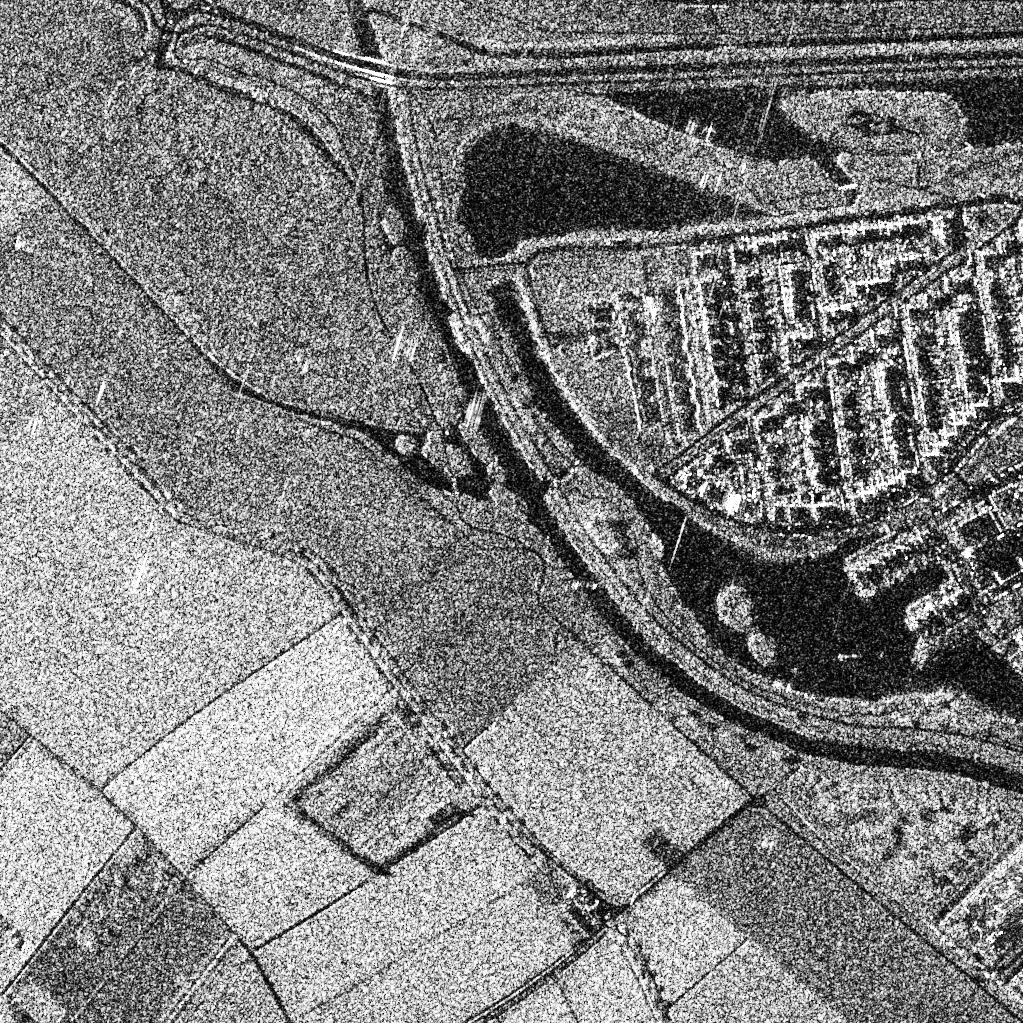
\includegraphics[width=55mm]{../Figures/PNG/Rotterdam_1024}\hskip1em
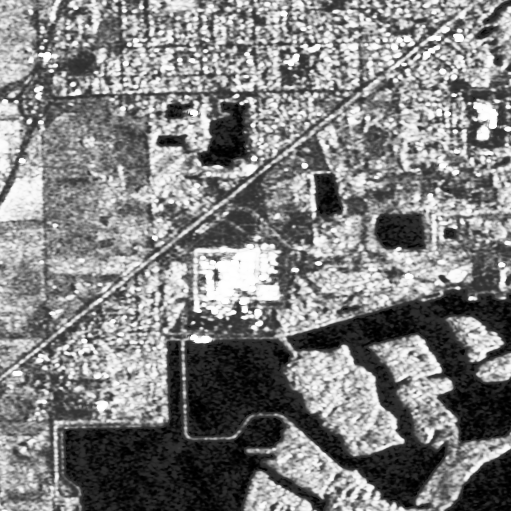
\includegraphics[width=55mm]{../Figures/PNG/lake_512}

Apart from the brightness, notice that different types of areas have distinct roughness.
\end{frame}

\begin{frame}{Statistical models}
The main models are the Gamma (suitable for fully-developed speckle) and
\(\mathcal{G}_I^0\) (able to describe roughness) distributions~\citep{Frery1997}. 

They are characterized by the probability
density functions (pdfs): 
\begin{align}
	f_Z(z;L, \mu\mid \Gamma_{\text{SAR}})&=\frac{L^L}{\Gamma(L)\mu^L}z^{L-1}\exp\left\{-Lz/\mu\right\} \mathbbm 1_{\mathbbm R_+}(z)\label{E:gamma1}\\
	\intertext{ and }
	f_Z(z; \alpha, \gamma, L \mid \mathcal{G}_I^0)&=\frac{L^L\Gamma(L-\alpha)}{\gamma^{\alpha}\Gamma(-\alpha)\Gamma(L)}\cdot\frac{z^{L-1}}{(\gamma+Lz)^{L-\alpha}} \mathbbm 1_{\mathbbm R_+}(z),\label{E:gi01}
\end{align} 
where \(\mu > 0\) is the mean, \(\gamma > 0\) is the scale,
\(\alpha < 0\) measures the roughness, \(L \geq 1\) is the number of
looks, \(\Gamma(\cdot)\) is the gamma function, and
\(\mathbbm 1_{A}(z)\) is the indicator function of the set \(A\).
\end{frame}

\begin{frame}{The statistical approach}
\begin{columns}
	\begin{column}{.63\linewidth}
{\includegraphics<1>[width=\linewidth]{../Figures/PDF/GammaGI0Densities}}
{\includegraphics<2>[width=\linewidth]{../Figures/PDF/GammaGI0DensitiesSemilog}}
	\end{column}
	\begin{column}{.3\linewidth}
	We need to identify the model that best describes the data.
	
	But it is a challenging task because
	\begin{itemize}
		\item Samples are small, and
		\item Parameter estimators are tricky.
	\end{itemize}
	\end{column}
\end{columns}
\end{frame}

\begin{frame}[standout]
\frametitle{Takeaways}
You may forget about the technical contents of this talk, but remember:
\begin{itemize}[<+->]
	\item No problem is too old to be revisited.
	\item The data statistical properties always bring valuable information.
	\item A careful mathematical manipulation often leads to new exciting results.
	\item Reproducibility goes a long way!
\end{itemize}
\end{frame}


\begin{frame}[allowframebreaks,allowdisplaybreaks]
\bibliographystyle{agsm}
\bibliography{references} 	
\end{frame}

\begin{frame}[standout]
\frametitle{The End}
\begin{columns}
	\begin{column}{.4\linewidth}
		\centering
		\includegraphics[width=.7\linewidth]{QRCode-WebPageVUW}\\	\includegraphics[width=\linewidth]{"Logo Offshore Reversed Landscape RGB"}
	\end{column}
	\begin{column}{.6\linewidth}
		Thanks for your kind attention!
		
		Questions?
	\end{column}
\end{columns}

\end{frame}

\end{document}
